\subsection{Pressure Treatment}

Applied mechanical pressure during the bonding phase can promote intimate
contact by elastically deforming surface asperities and closing residual
gaps at the interface \cite{mai2015, trinh2022}, as illustrated in
Figure~\ref{fig:pressure}. This mechanical assistance is particularly
relevant for wafers with insufficient flatness, where the van der Waals
attraction alone cannot provide enough energy to close macroscopic gaps
\cite{turner2006, kalk2014}. In those cases, the bonding condition can be
understood through an energy balance: bonding propagates when the reduction
in surface energy associated with the newly formed interface exceeds the
elastic strain energy stored in the deformed wafers. External pressure
shifts this balance in favor of bonding by forcing asperities into contact
\cite{turner2006, turner2002}.

For well-polished, optically flat wafers, however, the role of pressure is
more ambiguous. Since the bonding energy at room temperature is governed
primarily by the real area of contact---which is in turn dictated by
surface roughness at the nanoscale rather than by externally applied
load---additional mechanical pressure does not necessarily increase the
intrinsic bond energy \cite{miki2003, takagi1998}. In this regime, the
spontaneous van der Waals or hydrogen-bonding forces are already sufficient
to bring the surfaces into full intimate contact, and the bond energy is
ultimately limited by the surface chemistry and the density of interfacial
bonds, not by the mechanical load. This is consistent with the classical
observation that optically contacted surfaces adhere spontaneously without
any applied force \cite{possl1999}. External
pressure is therefore best understood as a means of extending the range of
acceptable wafer flatness rather than as a mechanism for strengthening an
already well-formed bond.

Pressure magnitude must nonetheless be optimized carefully, regardless of
wafer quality. Research on Borofloat~33 wafers demonstrates that a load of
\SI{0.07}{\mega\pascal} maximizes flexural strength; pressures beyond this
threshold introduce stress concentrations that cause premature failure
\cite{trinh2022}. Non-uniform pressure distributions pose additional
risks: stress-induced birefringence and permanent wavefront distortion can
compromise optical performance in precision devices \cite{bain2022,
wang2014}. High-precision applications therefore require well-planarized
pressure plates with peak-to-valley flatness on the order of micrometers,
fabricated from stiff materials such as technical ceramics \cite{birckigt2021}.

\begin{figure}[h]
\centering
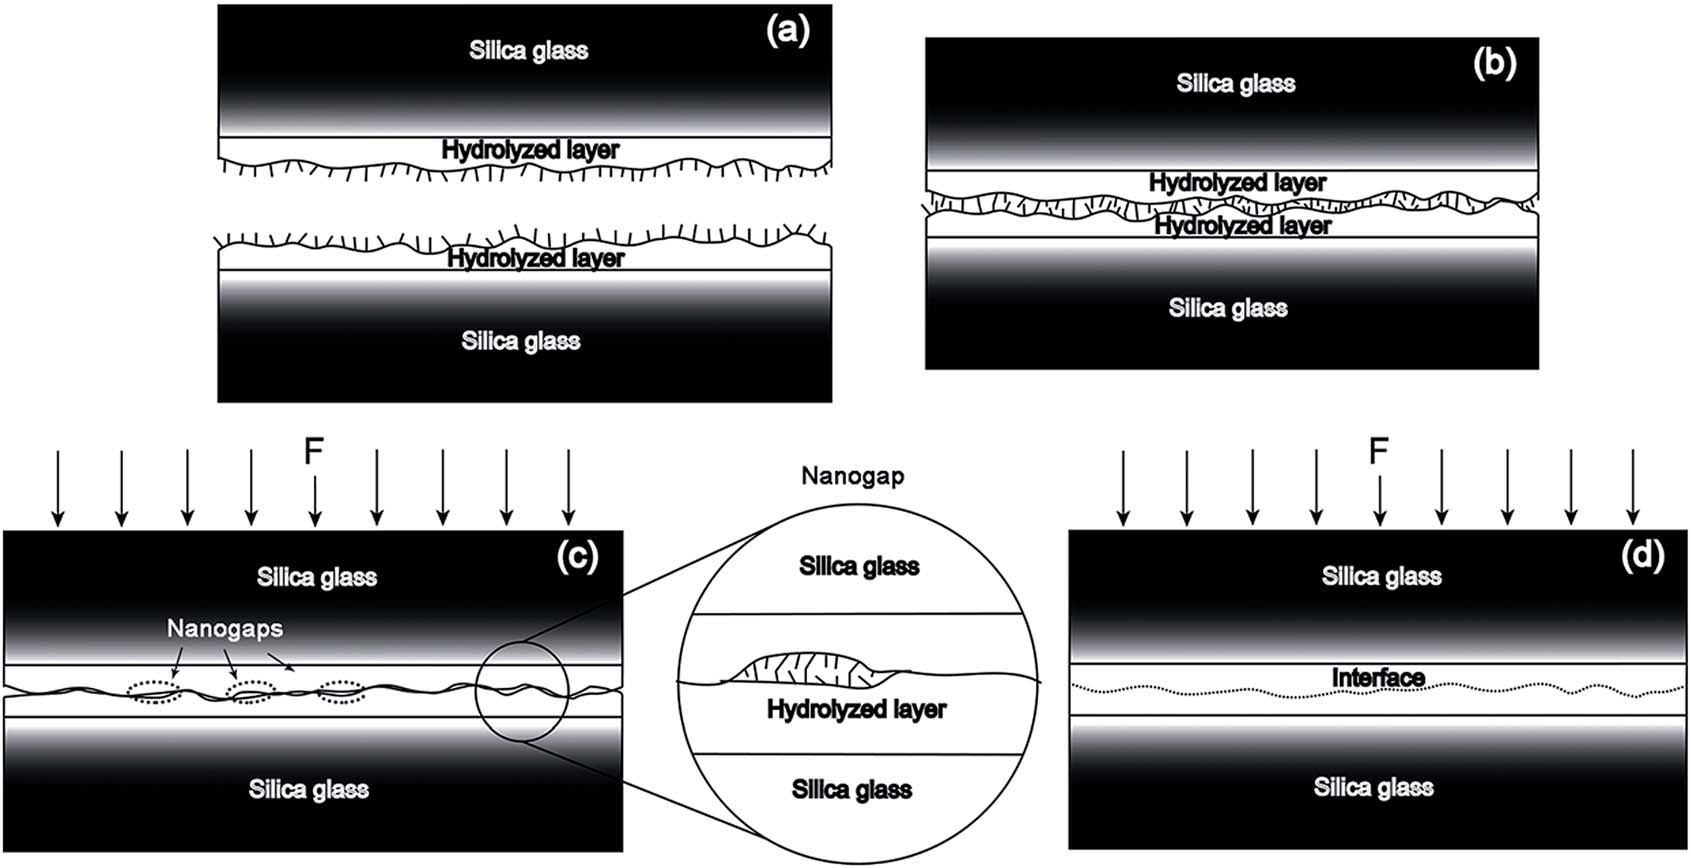
\includegraphics[width=0.8\linewidth]{Images/pressure.png}
\caption{Effect of applied pressure on the bonding process. Forces
    perpendicular to the interface suppress void formation by closing
    residual gaps between surface asperities. From \cite{mai2015}.}
\label{fig:pressure}
\end{figure}

Birckigt et al.\ \cite{birckigt2021} describe a setup in which convex and
concave pressure plates---with waviness of \SI{5}{\micro\meter} and
\SI{3}{\micro\meter}, respectively---promote radially outward propagation
of the contact front during the initial bonding phase
(Figure~\ref{fig:chucks}). This geometry mitigates the risk of void
entrapment and introduces radially symmetric residual stresses that are
more predictable and manageable than those arising from asymmetric loading.
A key insight from this work is that the geometry and flatness of the
pressure plates affect the contact-front dynamics independently of the
magnitude of the applied load, underscoring that pressure uniformity is
often more critical than pressure magnitude.

\begin{figure}[h]
\centering
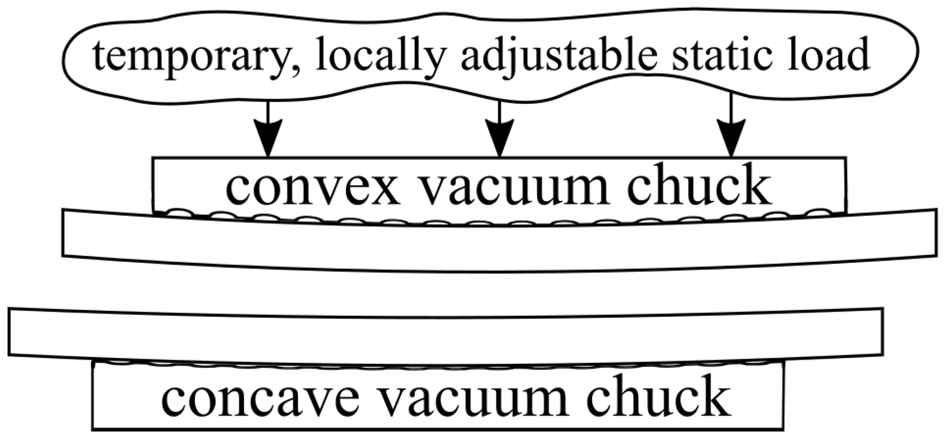
\includegraphics[width=0.6\linewidth]{Images/chucks.png}
\caption{Pressure plate geometry described by Birckigt et al.\
\cite{birckigt2021}. The curved profiles guide contact front propagation
    outward from the center, reducing the probability of interface void
    formation.}
\label{fig:chucks}
\end{figure}